
\let\textcircled=\pgftextcircled
\chapter{A brief introduction to Ardupilot} \label{chap:ardupilot}

\initial{A}s it was mentioned in Section \ref{sec:motivation}, it is intended to bring the technology developed within this project to the widest range of UAVs.
However, there exist in the market several families of controller boards (which mainly consist on a microcontroller or microprocessor, in charge of all the basic functions required for an stable flight) that can only be used with specific hardware and/or software, not being compatible with each other since they implement different communication protocols.
Furthermore, some manufacturers work with proprietary software, of which little information on the low-level functioning is available to the public.

It is clearly impractical to try to target all the existing standards for this project, so a compromise needs to be made.
The thesis will be elaborated for the Ardupilot family of controllers, for being the most widespread open-source\footnote{The software is being developed at GitHub: \url{https://github.com/ArduPilot/ardupilot}} alternative.
Some of the leading companies \cite{droneindustryinsights2016} in the sector actively support the Dronecode Project, of which Ardupilot is part, such as Intel, Qualcomm, Parrot, 3DR, Yuneec, AUAV, Walkera\ldots \cite{dronecode2016}

It is important nonetheless to clarify some concepts and features of any Ardupilot-equipped UAV.
More information can be found at \url{www.ardupilot.org}.

\section{Basic features} \label{sec:basics}

The most basic but important feature of the controller is to give control to the pilot over the vehicle.
There are several components that make this function possible.

Firstly, the pilot expresses the desired movements of the vehicle through a Radio Control (RC) transmitter, shown in Figure \ref{fig:RCtransmitter}.
The signal at 2.4 GHz is received by the RC receiver located in the vehicle, depicted in Figure \ref{fig:RCreceiver}.
Then the receiver translates the electromagnetic wave into several PWM (Pulse Width Modulation) signals, one for each input channel up to a maximum of 8 channels, which are inputted to the controller board.
However, for the primary control of the vehicle, only 4 channels are needed: throttle, roll, pitch and yaw.
The additional channels are used to control extra features such as the flight mode, the landing gear or the camera controls.

\begin{figure}[htbp]
	\centering
	\begin{subfigure}[b]{0.25\textwidth}
		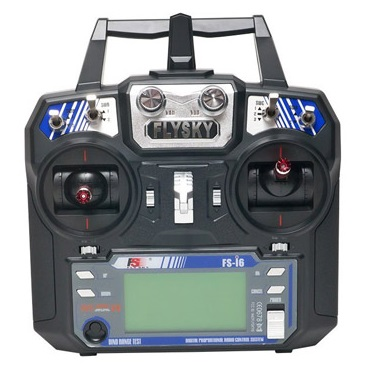
\includegraphics[width=\textwidth]{./figures/RCtransmitter.jpg}
		\caption{RC transmitter}
		\label{fig:RCtransmitter}
	\end{subfigure}
	\hspace{5mm}
	\begin{subfigure}[b]{0.3\textwidth}
		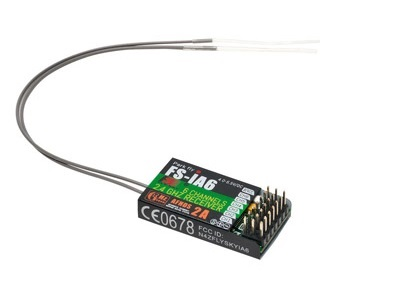
\includegraphics[width=\textwidth]{./figures/RCreceiver.jpg}
		\caption{RC receiver}
		\label{fig:RCreceiver}
	\end{subfigure}
	\caption{FlySky FS-i6 Remote Control (\footnotesize{\url{www.flyskyrc.com}})}
	\label{fig:rc}
\end{figure}

The second step is to translate the commands from the pilot into signals to the control elements of the vehicle.
These can vary depending on the type of vehicle (for example the yaw command affects the rudder in the case of a fixed-wing aircraft, the tail rotor collective control for a conventional helicopter or the differential throttle in the diagonals for a multicopter) but the underlying processes are similar.

Every Ardupilot controller board must have at least and Inertial Measurement Unit (IMU) consisting of a 3-axis accelerometer plus a 3-axis gyroscope for the state determination of the vehicle.
Additionally, a barometer, a GPS and other sensors can be integrated.
Hence, reading the pilot's commands from the RC receiver and the state of the vehicle from the IMU, the output to the control elements can be computed by some regular PID control loops (more information on the topic can be found at \cite{ogata2010}).
To the output pins of the controller board are connected the control elements, be it some servo-motors for the control surfaces of a fixed-wing aircraft or brushless motors with propellers for the case of a multicopter.
These elements are externally powered by the primary battery.

\section{Ardupilot as part of a UAS}

If Ardupilot wants to be used as a professional tool to enhance production or reduce costs, it can not rely on manual control only. 
For more advanced missions and proper calibration of vehicles with diverse configurations and physical properties, it is necessary to tweak the parameters that the control loops necessitate for their real-time computations.
It is in those cases when a Ground Control Station can become useful.
By connecting the vehicle to an external computer, the operator is no longer limited to the 8 input channels that the RC transmitter can provide.
Instead, the limit on the amount of information that the Ardupilot board can broadcast or absorb is only bound by the communication protocol that is implemented between the two.

For the Ardupilot ecosystem the protocol used is also open-source and receives the name of MAVlink\footnote{More information on the protocol can be found on \url{qgroundcontrol.org/mavlink/start}. The message definitions and generator code can be found at its GitHub repository \url{github.com/mavlink/mavlink/}} (MAV stands for Micro Aerial Vehicle).
Its open nature allows developers to create a very diverse set of software and applications to communicate with the UAV, from the widespread Mission Planner and APM planner, to versions that run on Android devices for on-the-field operation or developer-oriented libraries that run under Python, for example.

Another feature that is worth mentioning is the lightweight nature of the protocol, which not only permits the connection via USB cable, but also wirelessly through what is usually called a telemetry radio, which effectively is a serial transmission of data over a 433 MHz radio wave carrier.

An experienced operator can take advantage of all the mentioned features to receive real-time information on the state of the vehicle while it is on the air, and also to send high-level commands to the vehicle.
Those options will be further discussed in Section \ref{sec:advanced}.

\begin{figure}[htbp]
	\centering
	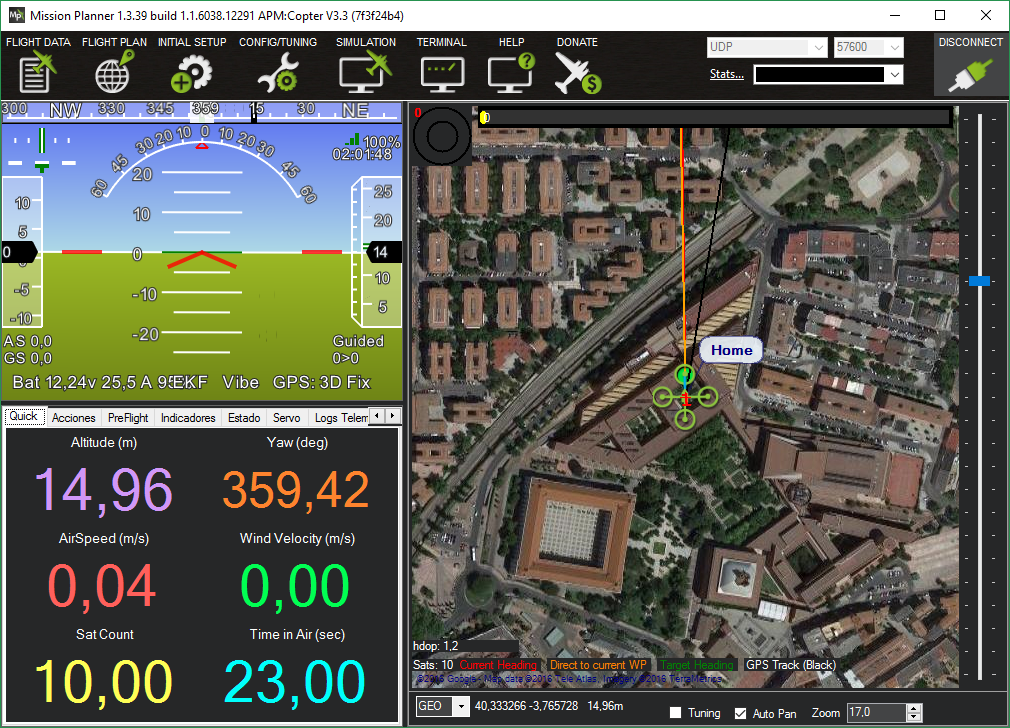
\includegraphics[width=\textwidth]{./figures/missionplanner.png}
	\caption{Screenshot of Mission Planner GCS, implementing the MAVlink protocol}
	\label{fig:missionplanner}
\end{figure}

\section{Advanced features}\label{sec:advanced}

For an Ardupilot UAV to be able to automate some missions and procedures there are some additional requirements.
Firstly, the IMU is appropriate for the evaluation of the vehicle's state variables, but the knowledge of its environment can only be acquired through absolute positioning sensors.
Those sensors are usually a GPS module for horizontal positioning and a barometer for altitude measurement.
Secondly, a wireless data-link provides a much more flexible way of interacting with the UAV during the execution of the mission.

\subsection{Flight modes}

Ardupilot has separated the mentioned advanced features in different flight modes, which can be activated with the 5$^{\text{th}}$ channel on the RC transmitter or from the GCS.
At the time of writing, there are 15 different flight modes, but just the most relevant ones for the project will be described here.
A summary of the most important features can be found in Table \ref{tab:modes}.

From this point onwards the concepts involving Ardupilot will be particularised for the quadcopter variant, since it is the type of aircraft that will be used for the prototype.
Similar information can be found for the rest of supported vehicle configurations, shown in Figure \ref{fig:vehicles}.

\begin{description}

	\item[\scshape Stabilize] 
		The default mode for manual control.
		Uses only the IMU data to control the flight.
		The pitch and roll channels define the Euler angles (instead of the rotation rate of Acrobatic mode) so that when the controls are released to neutral position, the vehicle will level off automatically.
		The yaw channel does control the yaw rate of the UAV instead, while for the throttle channel
		Ardupilot will not compensate for wind or other disturbances.

	\item[\scshape Altitude hold]
		Very similar to the Stabilize mode.
		The only difference is on the throttle channel, which controls the ascension rate instead of raw power transmitted to the motors.
		When the throttle stick is centered, the vehicle will hold the current altitude using the information measured by the onboard barometer.

	\item[\scshape Loiter]
		Incorporates the GPS data to the Altitude hold mode, making it possible for the UAV to compensate for wind and IMU drift.
		The pilot still has control on the vehicle similarly to Altitude hold but when the control sticks are released, the position will be kept within a 1 metre error (provided good quality GPS signal).

	\item[\scshape Auto]
		This mode allows to automate missions and procedures.
		With the help of a GCS application, such as the one shown in Figure \ref{fig:missionplanner}, the operator can click on a map to define waypoints and actions (take of, land, point to a certain direction, etc. are within the options) and save a data file to the vehicle's internal storage.
		Later, when the mode is activated, the vehicle will follow the predefined route without the need of direct input from the pilot.
		The throttle, yaw, pitch and roll controls will be disregarded when Auto mode is active, but the pilot can change the active mode at any time from the RC transmitter.

	\item[\scshape RTL (Return To Launch)]
		RTL mode is commonly used as a failsafe feature, when communication either with the pilot or the GCS is lost.
		It is a very specific version of the Auto mode that automatically starts the return to Home procedure, landing the vehicle exactly where it took off from.
		The Home location is defined as the point were the motors were initially armed (the arming procedure resembles the engine startup of a conventional aircraft: the motors will not spin unless the vehicle is armed)

	\item[\scshape Guided]
		The only difference between the Auto and the Guided modes is that whereas in the Auto mode the mission needs to be completely defined and uploaded to the vehicle before it is executed, the Guided mode allows for on-the-fly control of the vehicle from the GCS, taking complete advantage of the MAVlink commands over the telemetry link.
		This characteristic makes it very flexible for real-time development of applications.

		
\end{description}


\begin{table}[htbp]
\centering
\begin{tabular}{lm{3.1cm}ccm{3cm}} 
	\hline
	\bfseries Mode	& \bfseries Sensors used	& \bfseries Throttle	&	\bfseries Roll/Pitch	&	\bfseries Features	\\
	\hline
	Stabilize		&	IMU					&	Power			&	Euler angles		&	Fully manual			\\
	Altitude hold	&	IMU + Barometer		&	Ascension rate	&	Euler angles		&	Enhanced altitude control\\
	Loiter			&	IMU + Barometer + GPS&	Ascension rate	&	Euler angles		&	Disturbance rejection	\\
	Auto			&	IMU + Barometer + GPS&	No control		&	No control			&	Mission automation		\\
	RTL				&	IMU + Barometer + GPS&	No control		&	No control			&	Failsafe				\\
	Guided			&	IMU + Barometer + GPS&	No control		&	No control			&	Real-time commands		\\
	\hline
\end{tabular}
\caption{Summary of the relevant flight modes}
\label{tab:modes}
\end{table}



\begin{figure}[htbp]
	\centering
	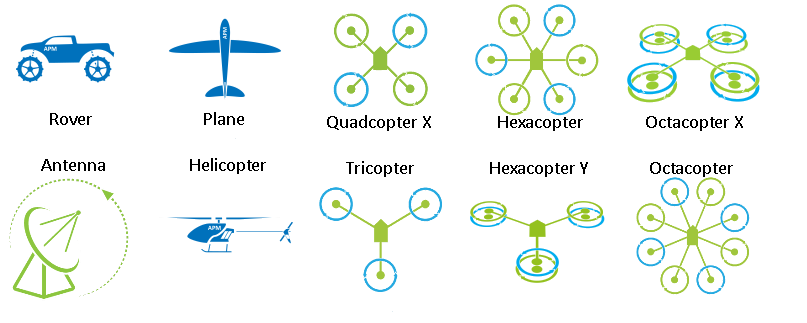
\includegraphics[width=\textwidth]{./figures/vehicles.png}
	\caption{Vehicle configurations supported by Ardupilot}
	\label{fig:vehicles}
\end{figure}


